%%%%%%%%%%%%%%%%%%%%%%%%%%%%%%%%%%%%%%%%%%%%%%%
%%%%%%%%%%%%%%%%%%%%%%%%%%%%%%%
\documentclass{l3deliverable}
%%%%%%%%%%%%%%%%%%%%%%%%%%%%%%%%%%%%%%%%%%%%%%%
%%%%%%%%%%%%%%%%%%%%%%%%%%%%%%%
\usepackage{graphicx}%
\usepackage{tabularx}%
\usepackage{url}%
\usepackage{usecasedescription}%
%%%%%%%%%%%%%%%%%%%%%%%%%%%%%%%%%%%%%%%%%%%%%%%
%%%%%%%%%%%%%%%%%%%%%%%%%%%%%%%
%% Check these macro values for appropriateness for your own document.
\title{Requirements Document}
\author{Ross Adam\\
Andrew Gardner\\
Nicole Kearns\\
Mamas Nicolaou\\
Asset Sarsengaliyev\\
}
\date{1st November 2012}
\deliverableID{D3}
\project{PSD3 Group Exercise 1}
\team{V}
\version{2.0}
%%%%%%%%%%%%%%%%%%%%%%%%%%%%%%%%%%%%%%%%%%%%%%%
%%%%%%%%%%%%%%%%%%%%%%%%%%%%%%%
\begin{document}
%%%%%%%%%%%%%%%%%%%%%%%%%%%%%%%%%%%%%%%%%%%%%%%
%%%%%%%%%%%%%%%%%%%%%%%%%%%%%%%
\maketitle
\tableofcontents
\newpage
%%%%%%%%%%%%%%%%%%%%%%%%%%%%%%%%%%%%%%%%%%%%%%%
%%%%%%%%%%%%%%%%%%%%%%%%%%%%%%%
%% Standard section for all documents
\section{Introduction}

\subsection{Identification}

Requirements specification for the internship management system for PSD3 team project.
\subsection{Related Documentation}

PSD3 Group Exercise Description \url{http://fims.moodle.gla.ac.uk/file.php/128/coursework/
psd3-ge-1-rev3278.pdf}\\
Deliverables Template \url{http://fims.moodle.gla.ac.uk/file.php/128/coursework/templates.zip}\\
PSD3 Course Notes \url{http://fims.moodle.gla.ac.uk/file.php/128/lecture-notes/notes-r3275.pdf}
\\
\subsection{Purpose and Description of Document}

The purpose of this document is to detail and explain the requirements collected for the
internship management system. This will include all actors within the system, their use cases, descriptions and suitable 
scenarios for the system.
%%%%%%%%%%%%%%%%%%%%%%%%%%%%%%%%%%%%%%%%%%%%%%%
%%%%%%%%%%%%%%%%%%%%%%%%%%%%%%%

\subsection{Document Status and Schedule}

\begin{center}{
\begin{tabular}{|c|c|c|c|}
\hline \textbf{Date} &\textbf{ Change} & \textbf{Version} & \textbf{Author}\\ 
\hline 25/10/2012 & Began Draft & 0.1 & All \\ 
\hline 30/10/2012 & Initial Draft Completed & 0.2 & All \\ 
\hline 10/11/2012 & Finalised for Submission & 0.3 & All\\ 
\hline 11/11/2012 & \textbf{Draft Submission Deadline} & 1.0 & All\\ 
\hline 19/11/2012 & Modified Section 4 & 1.1 & Nicole\\
\hline 20/11/2012 & Modified Non-Functional Requirements & 1.2 & Mamas Nicolaou\\
\hline 26/11/2012 & Modified the use case diagrams & 1.3 & Nicole\\
\hline 26/11/2012 & Modified the use case descriptions & 1.4 & Andrew\\
\hline 27/11/2012 & Modified the use case scenarios & 1.5 & Nicole\\
\hline 28/11/2012 & Minor modifications to all use cases & 1.6 & Andrew, Nicole, Mamas\\
\hline 28/11/2012 & Finalised for submission & 2.0 & Andrew, Mamas\\
\hline 29/11/2012 & \textbf{Final Submission Deadline} &2.0 & Andrew, Mamas\\ 
\hline 
\end{tabular} }
\end{center}

\section{Extended Problem Definition}
A system is needed to manage internship adverts posted by companies so that students can browse
through them and apply if they are interested.
In order for this system to be successful it requires a login mechanism, allowing a company
to submit and edit their adverts. Submitted adverts are then approved by the Course
Co-ordinator. If approved they will be made available for the students to see.
Applying will direct the student to the appropriate apply page belonging to the company. 
The Course Co-ordinator will remove any adverts that have been filled or whose deadlines have expired.\\
%%%%%%%%%%%%%%%%%%%%%%%%%%%%%%%%%%%%%%%%%%%%%%%
%%%%%%%%%%%%%%%%%%%%%%%%%%%%%%%
\section{System Scope}

%%%%%%%%%%%%%%%%%%%%%%%%%%%%%%%%%%%%%%%%%%%%%%%
%%%%%%%%%%%%%%%%%%%%%%%%%%%%%%%

\subsection{System Actors}
\textbf{Course Co-ordinator}: Responsible for the management of adverts on the system.\\
\textbf{Students}: Uses the system to browse available internship adverts and apply.\\
\textbf{Company}: Submits adverts for approval.\\

%%%%%%%%%%%%%%%%%%%%%%%%%%%%%%%%%%%%%%%%%%%%%%%
%%%%%%%%%%%%%%%%%%%%%%%%%%%%%%%

\subsection{Domain Model}

\begin{center}
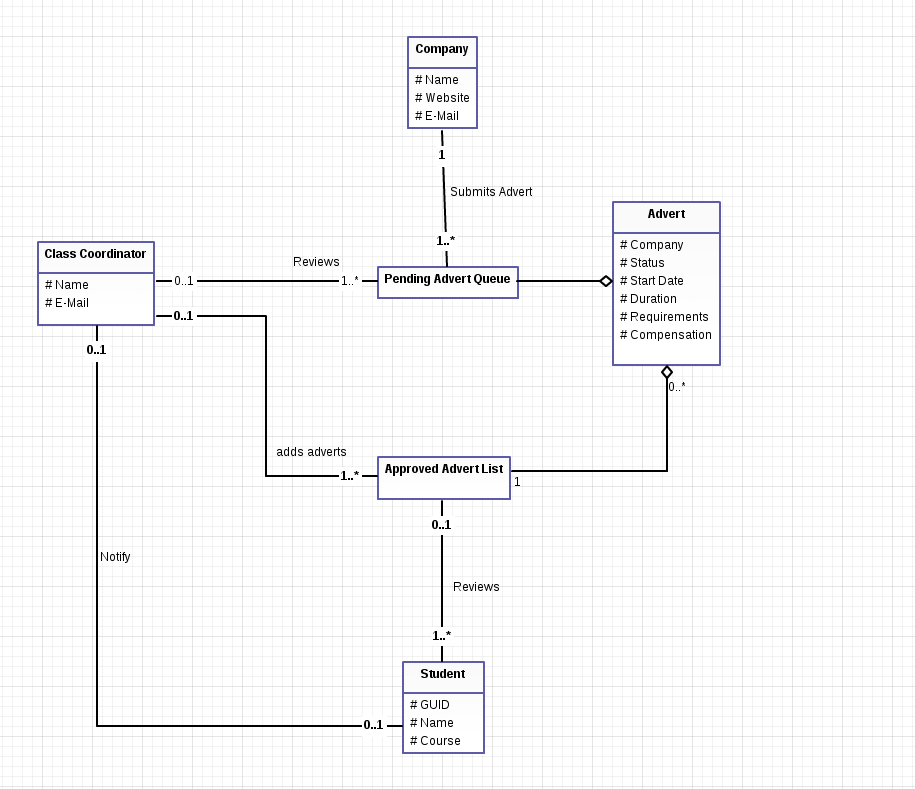
\includegraphics
[scale=0.7]
{img/UML.png}
\end{center}

%%%%%%%%%%%%%%%%%%%%%%%%%%%%%%%%%%%%%%%%%%%%%%%
%%%%%%%%%%%%%%%%%%%%%%%%%%%%%%%

\section{Use Case Descriptions}

This section describes the required functionality for the internship management system as four groups of related
use cases. The core use cases for the system are:\\

\textbf{Submission of internship advert by Company (Section 4.1):}
\begin{itemize}
\item Submit internship advert
\item Edit advert
\end{itemize}

\textbf{Review and approval of internship adverts by Course Co-ordinator (Section 4.2):}
\begin{itemize}
\item Review internship adverts
\item Approve internship advert
\end{itemize}

\textbf{Review of adverts by Student (Section 4.3):}
\begin{itemize}
\item View internship adverts
\item Apply for internship
\end{itemize}

\textbf{Notification of successful internship placement by Student (Section 4.4):}
\begin{itemize}
\item Notify of successful placement
\item Remove internship advert
\end{itemize}

\textbf{Common utility services (Section 4.5):}
\begin{itemize}
\item Login
\item Logout
\end{itemize}

\subsection{Submission of internship advert by Company}


\begin{center}
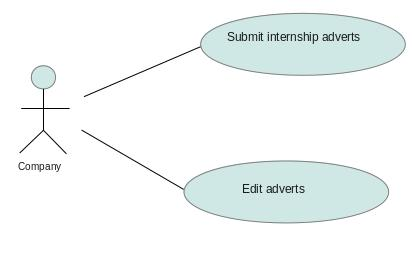
\includegraphics
[scale=0.7]
{img/Company.jpeg}
\end{center}

\begin{UseCaseTemplate}
\UseCaseLabel{Submit internship advert}
\UseCaseDescription{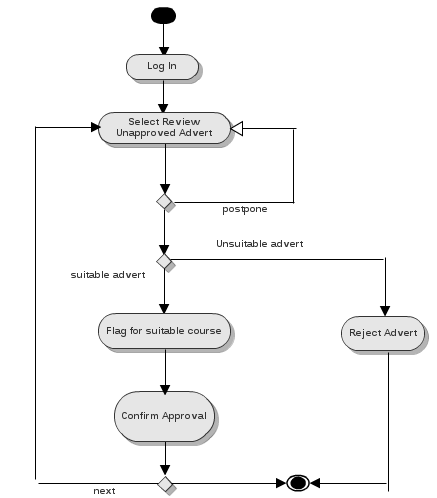
\includegraphics[scale=0.7]{img/SubmitAdvert.png}}
\UseCaseRationale{During the client interview we were given the requirement that a company must be able to submit internship adverts to the system in order for the students to view and apply for the placement.}
\UseCasePriority{Must have}
\UseCaseStatus{Not implemented}
\UseCaseActors{Company}
\UseCaseIncludes{Login, Logout}
\UseCaseConditions{\textbf{Post:} The advert is stored in the system, pending approval by the CC.}
\UseCaseNonFunctionalRequirements{Security}
\UseCaseScenarios{IBM are wanting to submit an internship advert to the system. They log in to the system using their designated username, IBM, fill out the submission form, confirm their submission and submit it to the system to eventually be approved by Timothy Storer, the current CC. IBM then logs out of the system.}
\UseCaseRisks{}
\end{UseCaseTemplate}

\begin{UseCaseTemplate}
\UseCaseLabel{Edit internship advert}
\UseCaseDescription{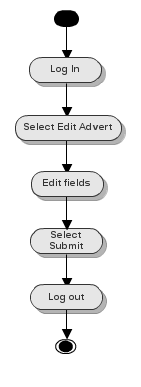
\includegraphics[scale=0.7]{img/EditAdvert.png}}
\UseCaseRationale{During the stakeholder panel meeting the need for companies to be able to edit pending approval adverts was clarified to be a requirement.}
\UseCasePriority{Must Have}
\UseCaseStatus{Not implemented}
\UseCaseActors{Company}
\UseCaseIncludes{Login, Logout}
\UseCaseConditions{\textbf{Pre:} Company's advert must currently be pending approval by the CC.}
\UseCaseNonFunctionalRequirements{Data Consistency}
\UseCaseScenarios{IBM realise that the advert they have previously submitted contains the wrong starting date. They log in to the system, select the relevant advert and section they want to edit and correct the starting date. They confirm their changes and then log out.}
\UseCaseRisks{During client interview we were told that this probably wouldn't be needed, yet during the stakeholder panel meeting it was made clear that it was a valid requirement.}
\end{UseCaseTemplate}

\subsection{Review and approval of internship adverts by Course Co-ordinator}


\begin{center}
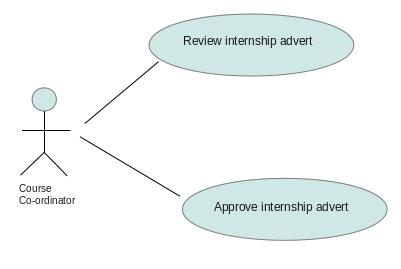
\includegraphics
[scale=0.7]
{img/CourseCoordinator.jpeg}
\end{center}


\begin{UseCaseTemplate}
\UseCaseLabel{Review internship adverts}
\UseCaseDescription{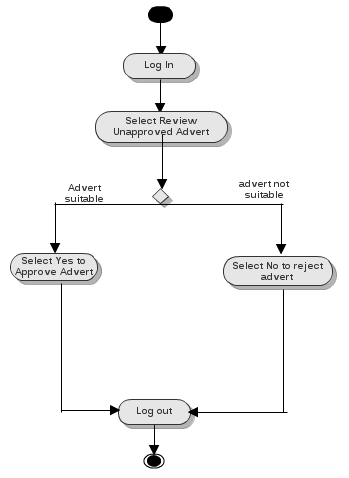
\includegraphics[scale=0.7]{img/ReviewAdvert.png}}
\UseCaseRationale{During the client interview we verified that it was essential for the CC to have the ability to review adverts.}
\UseCasePriority{Must have}
\UseCaseStatus{Not implemented}
\UseCaseActors{Course Co-ordinator}
\UseCaseIncludes{Login, Logout}
\UseCaseConditions{\textbf{Pre:} Must have advert(s) pending approval on system.}
\UseCaseNonFunctionalRequirements{Data Consistency}
\UseCaseScenarios{Timothy Storer, the current CC, logs in to the system with his GUID and views all pending adverts submitted to the system and decides whether or not each internship is suitable for student review.}
\UseCaseRisks{}
\end{UseCaseTemplate}
\begin{UseCaseTemplate}

\UseCaseLabel{Approve internship advert}
\UseCaseDescription{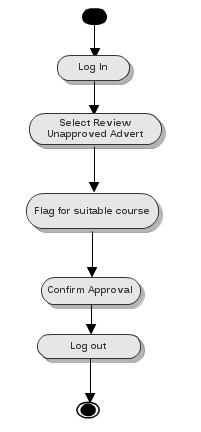
\includegraphics[scale=0.7]{img/ApproveAdverts.png}}
\UseCaseRationale{During the client interview we verified that it was essential for the CC to have the ability to approve adverts.}
\UseCasePriority{Must have}
\UseCaseStatus{Not implemented}
\UseCaseActors{Course coordinator}
\UseCaseIncludes{Login, Logout}
\UseCaseConditions{\textbf{Pre:} Must have advert(s) pending approval on system. \textbf{Post:} Approved advert now available for student viewing}
\UseCaseNonFunctionalRequirements{Data Consistency}
\UseCaseScenarios{After having reviewed an internship advert from IBM, Timothy Storer, the current CC, decides that the advert is suitable. He specifies what degree structure (CS/SE/ESE) it's suitable for and approves the advert for later student viewing.}
\UseCaseRisks{}
\end{UseCaseTemplate}

\subsection{Review of adverts by Student} %%%%%%%%%%%%%%


\begin{center}
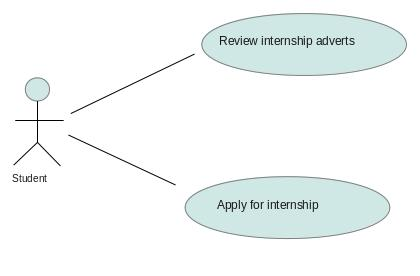
\includegraphics
[scale=0.7]
{img/Student.jpeg}
\end{center}


\begin{UseCaseTemplate}
\UseCaseLabel{View internship adverts}
\UseCaseDescription{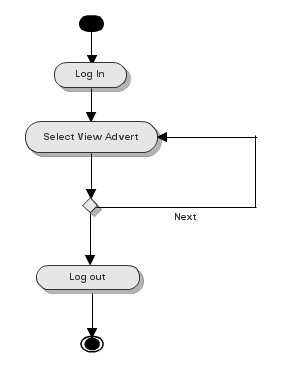
\includegraphics[scale=0.7]{img/StudentViewAdvert.png}}
\UseCaseRationale{During the client interview we verified that it was essential for students to have the ability to view adverts.}
\UseCasePriority{Must Have}
\UseCaseStatus{Not Implemented}
\UseCaseActors{Student}
\UseCaseIncludes{Login, Logout}
\UseCaseConditions{\textbf{Pre:} Must have advert(s) approved by the CC.}
\UseCaseNonFunctionalRequirements{User Concurrency, Security, Number of Adverts}
\UseCaseScenarios{Jim, a 3rd year Software Engineering student, wants to see if there is any suitable internships available that he might apply to. He logs into the system and selects the option that allows him to view the currently available internships.}
\UseCaseRisks{}
\end{UseCaseTemplate}

\begin{UseCaseTemplate}
\UseCaseLabel{Apply for internship}
\UseCaseDescription{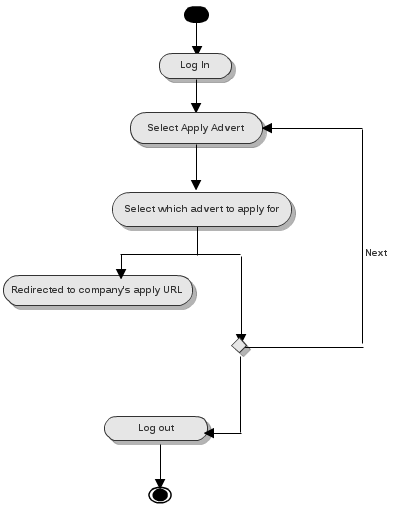
\includegraphics[scale=0.7]{img/StudentApply.png}}
\UseCaseRationale{During the interview the client told us that this would be a desirable feature to have but perhaps not essential.}
\UseCasePriority{Could Have}
\UseCaseStatus{Not Implemented}
\UseCaseActors{Student}
\UseCaseIncludes{Login, View internship adverts, Logout}
\UseCaseConditions{\textbf{Pre:} Must have advert(s) approved by the CC.}
\UseCaseNonFunctionalRequirements{User Concurrency, Security, Number of Adverts}
\UseCaseScenarios{Jim, the 3rd year Software Engineering student, wants to apply for the IBM internship that he saw whilst reviewing the available internships. He selects the Apply option, chooses the IBM internship and confirms his selection. Jim's browser then directs him to IBM's apply page on their website.}
\UseCaseRisks{The stakeholder panel meeting somewhat contradicted what we had gathered from our client interview, saying that applying through the system itself would be outwith the system scope. However, we felt that having the browser open the company's own apply URL was a reasonable compromise.}
\end{UseCaseTemplate}

\subsection{Notification of successful internship placement by student}

\begin{center}
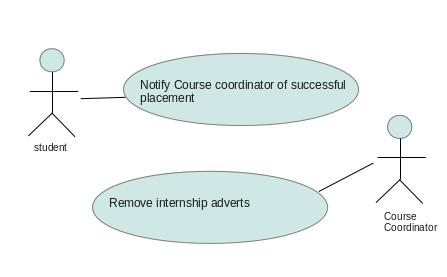
\includegraphics
[scale=0.7]
{img/Section4.jpeg}
\end{center}


\begin{UseCaseTemplate}
\UseCaseLabel{Notify of successful placement}
\UseCaseDescription{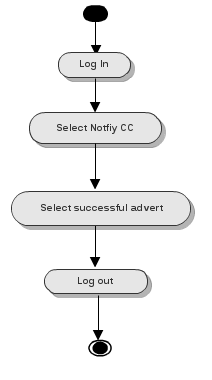
\includegraphics[scale=0.7]{img/NotifyPlacement.png}}
\UseCaseRationale{During the client interview we were told that allowing students to notify the CC of a successful placement was a requirement.}
\UseCasePriority{Should have}
\UseCaseStatus{Not Implemented}
\UseCaseActors{Student}
\UseCaseIncludes{Login, Logout}
\UseCaseConditions{\textbf{Pre:} The advert for the placement position that was taken must be still
visible on the system.}
\UseCaseNonFunctionalRequirements{User Concurrency, Security}
\UseCaseScenarios{Jim, the 3rd year Software Engineering student, has successfully obtained an internship at his company of choice, IBM. He logs in to the system in order to notify Timothy Storer, the current Course Co-ordinator, that he has got the placement. He selects the relevant option and selects the IBM placement to notify the Course Co-ordinator.}
\UseCaseRisks{The stakeholder panel meeting left this requirement somewhat abiguous but we didn't feel it was outwith the system scope.}
\end{UseCaseTemplate}

\begin{UseCaseTemplate}
\UseCaseLabel{Remove internship advert}
\UseCaseDescription{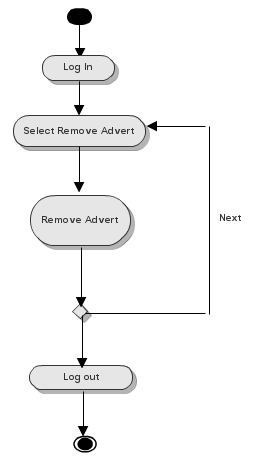
\includegraphics[scale=0.7]{img/RemoveAdvert.png}}
\UseCaseRationale{During our client interview we gathered that the CC must be able to remove adverts that were no longer available or had passed the deadline.}
\UseCasePriority{Must have}
\UseCaseStatus{Not implemented}
\UseCaseActors{Course Co-ordinator}
\UseCaseIncludes{Login, Logout}
\UseCaseConditions{\textbf{Pre:} Course Co-ordinator has recieved a notification to say the placement has been filled.}
\UseCaseNonFunctionalRequirements{Data Consistency}
\UseCaseScenarios{Timothy Storer, the current Course Co-ordinator, receives a notification that Jim the SE student has secured a placement with IBM. Timothy logs in to the system, finds and selects the IBM advert, and removes it from the system.}
\UseCaseRisks{}
\end{UseCaseTemplate}

\subsection{Common utility services}

\begin{UseCaseTemplate}
\UseCaseLabel{Login}
\UseCaseDescription{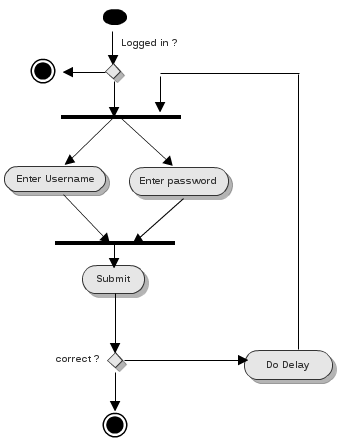
\includegraphics[scale=0.7]{img/Login.png}}
\UseCaseRationale{Logging in was ascertained to be a requirement both from client interview and stakeholder panel meeting.}
\UseCasePriority{Must have}
\UseCaseStatus{Not implemented}
\UseCaseActors{Company, Students, Course Co-ordinator}
\UseCaseIncludes{}
\UseCaseConditions{\textbf{Pre:} User should not be already logged in to the system.}
\UseCaseNonFunctionalRequirements{Security, User Concurrency}
\UseCaseScenarios{Jim, the 3rd year Softare Engineering student, wishes to access the internship management system. Knowing his GUID and password he logs in to the system.}
\UseCaseRisks{}
\end{UseCaseTemplate}

\begin{UseCaseTemplate}
\UseCaseLabel{Logout}
\UseCaseDescription{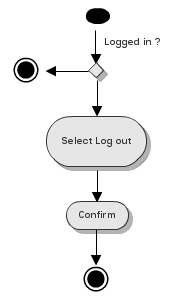
\includegraphics[scale=0.7]{img/Logout.png}}
\UseCaseRationale{Logging out was ascertained to be a requirement both from client interview and stakeholder panel meeting.}
\UseCasePriority{Must Have}
\UseCaseStatus{Not implemented}
\UseCaseActors{Company, Students, Course Coordinator}
\UseCaseIncludes{Login}
\UseCaseConditions{\textbf{Pre:} User must be currently logged in to the system.}
\UseCaseNonFunctionalRequirements{}
\UseCaseScenarios{Jim, the 3rd year software engineering student, after browsing the available adverts on the system but finding nothing suitable, wishes to log out of the system. He selects log out and his subsequently logged out of the system.}
\UseCaseRisks{}
\end{UseCaseTemplate}

%%%%%%%%%%%%%%%%%%%%%%%%%%%%%%%%%%%%%%%%%%%%%%%
%%%%%%%%%%%%%%%%%%%%%%%%%%%%%%%
\section{Non Functional Requirements}

\begin{itemize}
\item User Concurrency: The system should be available to all Students of the School of Computing Science. A large number of users might want to use the system at the same time so the system should be able to handle a large number of users at once.
\item Data Consistency: The system must maintain data accuracy and integrity throughout the sytem's use to ensure that each user observes a consistent view of the data despite any changes made by other users.
\item Security: Students and Course Co-ordinator should be able to log in with their GUIDs and passwords which would be the same used for other University of Glasgow websites such as Moodle and MyCampus. Employers who wish to use the system to post internship adverts will need to be provided with new usernames and passwords in order to use the system.
\item Number of Adverts: The system must be able to handle an unlimited number of adverts. Any number of companies might offer placement opportunities for students each year therefore the number of adverts that can be posted on the system must not be limited.
\end{itemize}

%%%%%%%%%%%%%%%%%%%%%%%%%%%%%%%%%%%%%%%%%%%%%%%
%%%%%%%%%%%%%%%%%%%%%%%%%%%%%%%
\section{Summary}

A company should upload their adverts to the system. The course coordinator will review
all adverts posted to the system and determine whether or not they are appropriate for the
students. If appropriate, the CC makes the advert available for the students to browse. If a student
wants to apply for an advert, they will be redirected to the company's website or apply through their website. If
a student successfully secures a placement, they must notify the Course Co-ordinator. The Course Co-ordinator will then remove the advert from the system if all placements have been filled or if the advert has passed the deadline.

%%%%%%%%%%%%%%%%%%%%%%%%%%%%%%%%%%%%%%%%%%%%%%%
%%%%%%%%%%%%%%%%%%%%%%%%%%%%%%%
\appendix

\section{Glossary}
CC - Course Co-ordinator\\
PSD - Professional Software Development

\section{Stakeholder Interview Documentation}

Key points we got from our interview with the client are:

\begin{itemize}
\item The company does not directly interact with the system.
\item The Course Coordinator will review adverts sent via email and if they are suitable, would
then be posted on the system.
\item When applying for internships, students will be redirected to the company website or given
an email address in order to send in their CV.
\item Students will notify the CC of a successful placement.
\item Once a student has accepted a placement, the advert is taken off the system.
\end{itemize}

\section{Stakeholder Panel Documentation}

Originally, we were informed that the company would not interact with the system, all adverts
would be submitted via email to the course coordinator. However, at the stakeholder meeting
it was clarified that the company would interact with the system. The company will be given a
username and password and will be able to post their adverts directly to the system. They will
have a to fill out a standard form with all the relevant information before submitting the advert.
The course coordinator will then review it to determine whether or not it is relevant for the
students. If so, the adverts is made available to the students.
%%%%%%%%%%%%%%%%%%%%%%%%%%%%%%%%%%%%%%%%%%%%%%%
%%%%%%%%%%%%%%%%%%%%%%%%%%%%%%%
\end{document}
%%%%%%%%%%%%%%%%%%%%%%%%%%%%%%%%%%%%%%%%%%%%%%%
%%%%%%%%%%%%%%%%%%%%%%%%%%%%%%%

